\documentclass[12pt]{book}
%\usepackage{fontspec}
\usepackage{polyglossia}
\usepackage{xcolor}
\definecolor{BrickRed}{RGB}{146,18,6}
\setdefaultlanguage{english}
\setotherlanguages{french,russian,greek,german,latin,polish,italian,dutch,bulgarian}
\setmainfont{IrradiantVariable}[
    ItalicFont =         {*-Italic},
    BoldFont =           {*},
    BoldItalicFont =     {*-Italic},
    Renderer = Harfbuzz,
    SizeFeatures={
      {Size=-6.5, OpticalSize=6},
      {Size=6.5-7.5, OpticalSize=7},
      {Size=7.5-8.5, OpticalSize=8},
      {Size=8.5-9.5, OpticalSize=9},
      {Size=9.5-10.5, OpticalSize=10},
      {Size=10.5-11.5, OpticalSize=11},
      {Size=11.5-12.5, OpticalSize=12},
      {Size=12.5-13.5, OpticalSize=13},
      {Size=13.5-14.5, OpticalSize=14},
      {Size=14.5-15.5, OpticalSize=15},
      {Size=15.5-16.5, OpticalSize=16},
      {Size=16.5-17.5, OpticalSize=17},
      {Size=17.5-, OpticalSize=18},
    },
    BoldFeatures={
      {Size=-6.5, OpticalSize=6, Weight=700},
      {Size=6.5-7.5, OpticalSize=7, Weight=700},
      {Size=7.5-8.5, OpticalSize=8, Weight=700},
      {Size=8.5-9.5, OpticalSize=9, Weight=700},
      {Size=9.5-10.5, OpticalSize=10, Weight=700},
      {Size=10.5-11.5, OpticalSize=11, Weight=700},
      {Size=11.5-12.5, OpticalSize=12, Weight=700},
      {Size=12.5-13.5, OpticalSize=13, Weight=700},
      {Size=13.5-14.5, OpticalSize=14, Weight=700},
      {Size=14.5-15.5, OpticalSize=15, Weight=700},
      {Size=15.5-16.5, OpticalSize=16, Weight=700},
      {Size=16.5-17.5, OpticalSize=17, Weight=700},
      {Size=17.5-, OpticalSize=18, Weight=700},
    },
    BoldItalicFeatures={
      {Size=-6.5, OpticalSize=6, Weight=700},
      {Size=6.5-7.5, OpticalSize=7, Weight=700},
      {Size=7.5-8.5, OpticalSize=8, Weight=700},
      {Size=8.5-9.5, OpticalSize=9, Weight=700},
      {Size=9.5-10.5, OpticalSize=10, Weight=700},
      {Size=10.5-11.5, OpticalSize=11, Weight=700},
      {Size=11.5-12.5, OpticalSize=12, Weight=700},
      {Size=12.5-13.5, OpticalSize=13, Weight=700},
      {Size=13.5-14.5, OpticalSize=14, Weight=700},
      {Size=14.5-15.5, OpticalSize=15, Weight=700},
      {Size=15.5-16.5, OpticalSize=16, Weight=700},
      {Size=16.5-17.5, OpticalSize=17, Weight=700},
      {Size=17.5-, OpticalSize=18, Weight=700},
    },
    % StylisticSet=8,
    ]
\newfontfamily{\stdfont}{IrradiantVariable}[
    ItalicFont =         {*-Italic},
    BoldFont =           {*},
    BoldItalicFont =     {*-Italic},
    Renderer = Harfbuzz,
    SizeFeatures={
      {Size=-6.5, OpticalSize=6},
      {Size=6.5-7.5, OpticalSize=7},
      {Size=7.5-8.5, OpticalSize=8},
      {Size=8.5-9.5, OpticalSize=9},
      {Size=9.5-10.5, OpticalSize=10},
      {Size=10.5-11.5, OpticalSize=11},
      {Size=11.5-12.5, OpticalSize=12},
      {Size=12.5-13.5, OpticalSize=13},
      {Size=13.5-14.5, OpticalSize=14},
      {Size=14.5-15.5, OpticalSize=15},
      {Size=15.5-16.5, OpticalSize=16},
      {Size=16.5-17.5, OpticalSize=17},
      {Size=17.5-, OpticalSize=18},
    },
    BoldFeatures={
      {Size=-6.5, OpticalSize=6, Weight=700},
      {Size=6.5-7.5, OpticalSize=7, Weight=700},
      {Size=7.5-8.5, OpticalSize=8, Weight=700},
      {Size=8.5-9.5, OpticalSize=9, Weight=700},
      {Size=9.5-10.5, OpticalSize=10, Weight=700},
      {Size=10.5-11.5, OpticalSize=11, Weight=700},
      {Size=11.5-12.5, OpticalSize=12, Weight=700},
      {Size=12.5-13.5, OpticalSize=13, Weight=700},
      {Size=13.5-14.5, OpticalSize=14, Weight=700},
      {Size=14.5-15.5, OpticalSize=15, Weight=700},
      {Size=16.5-17.5, OpticalSize=17, Weight=700},
      {Size=17.5-, OpticalSize=18, Weight=700},
    },
    BoldItalicFeatures={
      {Size=-6.5, OpticalSize=6, Weight=700},
      {Size=6.5-7.5, OpticalSize=7, Weight=700},
      {Size=7.5-8.5, OpticalSize=8, Weight=700},
      {Size=8.5-9.5, OpticalSize=9, Weight=700},
      {Size=9.5-10.5, OpticalSize=10, Weight=700},
      {Size=10.5-11.5, OpticalSize=11, Weight=700},
      {Size=11.5-12.5, OpticalSize=12, Weight=700},
      {Size=12.5-13.5, OpticalSize=13, Weight=700},
      {Size=13.5-14.5, OpticalSize=14, Weight=700},
      {Size=14.5-15.5, OpticalSize=15, Weight=700},
      {Size=15.5-16.5, OpticalSize=16, Weight=700},
      {Size=16.5-17.5, OpticalSize=17, Weight=700},
      {Size=17.5-, OpticalSize=18, Weight=700},
    },
    % StylisticSet=8,
    ]


\usepackage{microtype}
\raggedbottom
%\newfontfamily\cyrillicfont[Script=Cyrillic]{IrradiantVariable}
%\newfontfamily\greekfont[Script=Greek]{IrradiantVariable}
    \newcommand{\cyrillicfont}{\stdfont}
    \newcommand{\greekfont}{\stdfont}
    \newcommand{\germanfont}{\stdfont}
\tolerance=2000
\linespread{1.15}
\usepackage{graphicx}
\usepackage{lettrine}
\usepackage{hanging}
\newcommand{\vnum}[1]{{\addfontfeature{VerticalPosition=Superior}#1}}
\newcommand{\russ}[1]{\textrussian{\cyrillicfont#1}}
\newcommand{\grek}[1]{\textgreek{\greekfont\addfontfeature{Weight=400}#1}}
\newcommand{\germ}[1]{\textgerman{\germanfont#1}}
\newcommand{\frit}[1]{\textfrench{\itshape #1}}
\newcommand{\latn}[1]{\textlatin{\itshape\addfontfeatures{Ligatures=Historic,
    Weight=500,StylisticSet=8}#1}}
\begin{document}

\begin{titlepage}
\hrulefill\\
\Huge \centering \textcolor{BrickRed}{Irradiant} \\[1cm]
\huge \centering A modern antiqua typeface \\[1cm]
\large \centering by {\addfontfeature{Letters=SmallCaps,Weight=500}Peter S. Baker}\\[1cm]
\huge\centering {\itshape sampler and feature list} \\
\hrulefill
\end{titlepage}
\cleardoublepage

\section*{About the font}

Irradiant is based on two early typefaces by Francesco Griffo
(1450–1518), who worked for the Venetian publisher Aldus Manutius. The
first is the roman typeface used in \textit{Hypnerotomachia Poliphili}
(1499), a book famous for the beauty of its type, layout, and
illustrations; the second is the italic used in the Aldine Virgil of
1501, the first book to be set entirely in italics.

\begin{center}
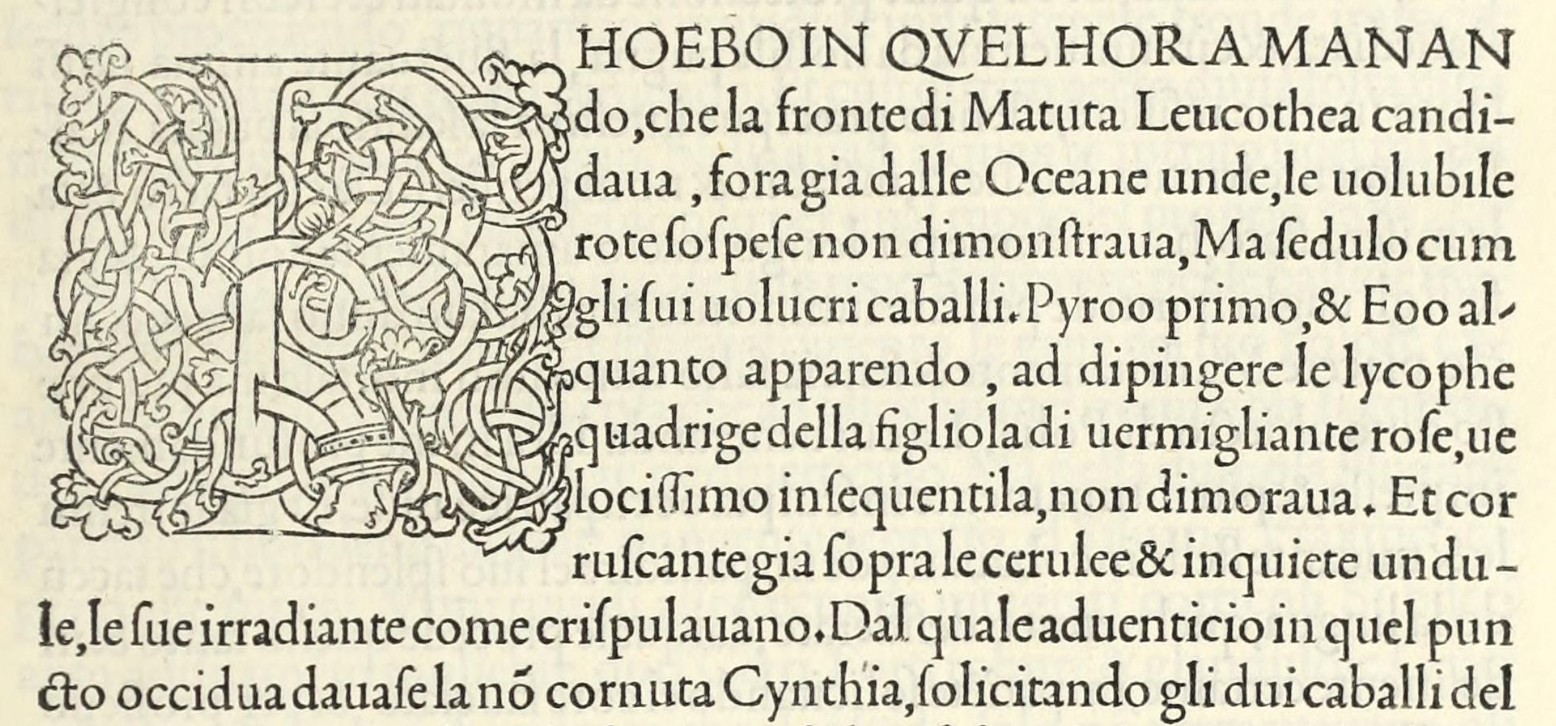
\includegraphics[width=0.6\textwidth]{hypnerotomachia_sample}\\[1ex]

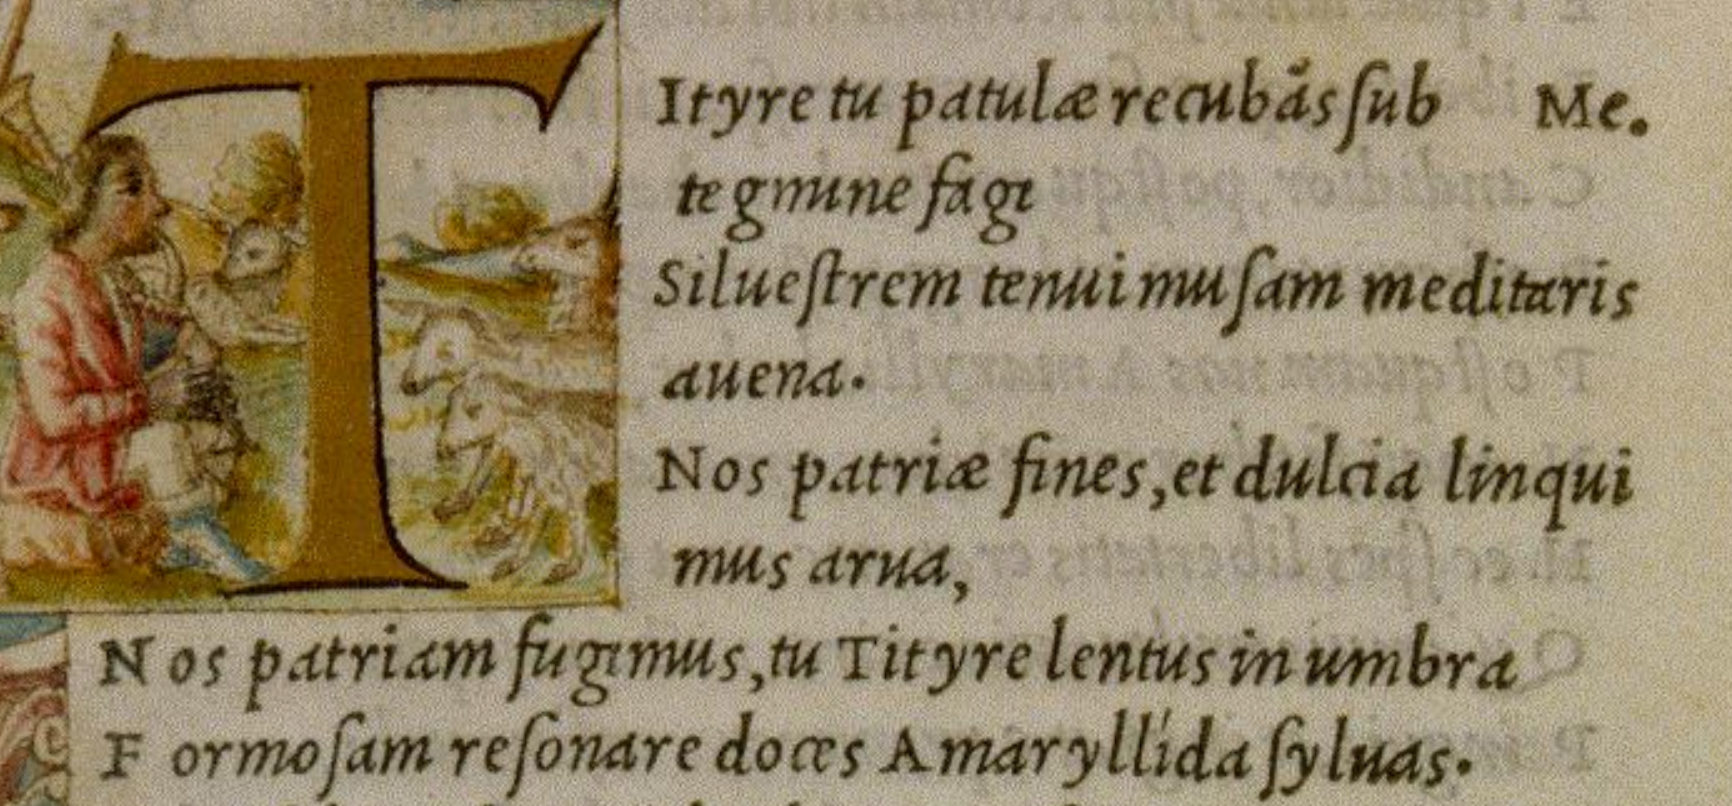
\includegraphics[width=0.6\textwidth]{Virgil_sample}
\end{center}

Despite its origins, Irradiant is not exactly a revival. Many changes,
both great and small, have been made to render the design suitable for modern
applications. Irradiant contains a Greek script that is very different
from Griffo's Greek types, being both modernized and designed to harmonize
with Irradiant's Latin letters. It also covers the Cyrillic script, for which 
Griffo’s types provide no model at all.

With its low contrast and gentle curves, Irradiant has an informal look, 
making it suitable for fiction, magazines, and most websites.
It covers over 300 languages, comes in both variable and static versions,
and has a number of OpenType features (for which see page 15).

\section*{Early modern English, mixed sizes and styles}

\noindent\textit{The Author begins his} Hypnerotomachia, \textit{to set
  down the hour and time when in his sleep it seemed to him that
  he was in a quiet solitary desert, and uninhabited plain, and
  from thence afterward how he entered unadvisedly before he was
  aware, with great fear, into a dark, obscure, and unfrequented
  wood.}

\begin{center}
  \textsc{The description of the morning.}
\end{center}

\lettrine[lines=5, loversize=0.1, findent=5pt, nindent=0em, image=true]{W}{hat hour} as \textit{Phœbus}\footnote{Phœbus the Sun.} issuing
forth did beautify with brightness the forehead of
\textit{Leucothea},\footnote{Leucothea the morning.} and appearing out
of the Ocean waves, not fully showing his turning wheels, that had
been hung up, but speedily with his swift horses \textit{Pyrous} \&
\textit{Eous}\footnote{Pyr \& Eo, the horses of the Sun.} hastening
his course, and giving a tincture to the Spider’s webs among the
green leaves and tender prickles of the Vermillion Roses, in the
pursuit whereof he showed himself most swift \& glistering, now upon
the never resting and still moving waves, he crisped up his irradiant
hair.

Upon whose uprising, even at that instant, the unhorned Moon
dismounted herself, loosing from her Chariot her two horses, the one
white and the other brown, and drew to the Horizon\footnote{Horizon
  a circle dividing the half sphere of the firmament from the other
  half which we do not see.} different from the
Hemisphere\footnote{Hemisphere is half the compass of the visible
  heaven.} from whence she came.

And whenas the mountains and hills were beautiful, and the
northeast winds had left off to make barren with the sharpness of
their blasts the tender sprigs to disquiet the moving reeds, the
fenny Bullrush, and weak Cyprus, to torment the folding Vines, to
trouble the bending Willow, and to break down the brittle Fir
boughs, under the horns of the lascivious Bull, as they do in
winter.

At that very hour, as the diverse coloured flowers and green meads,
at the coming of the sun of \textit{Hyperion}\footnote{Hyperion the Sun.}
fear not his burning heat, being bedewed and sprinkled with the
Crystalline tears of the sweet morning, whenas the
Halcyons\footnote{Halcyons are certain birds which building near the
  shore upon the waves there will be no storm until the young be
  hatched.} upon the level waves of the still, calm, and quiet
flowing seas do build their nests in sight of the sandy shore,
whereas the sorrowful Ero with scalding sighs did behold the
dolorous and ungrate departure of her swimming
\textit{Leander}.\footnote{Leander a young man of Abydos, who in swimming over
  Hellespont (a narrow sea by Byzantium, which parts Europe from Asia)
  to Sestus, was in the sight of his lover Ero of Sestus drowned,
  which she seeing, threw herself down into the sea, and died with
  him.}

I, lying upon my bed, an opportune and meet friend to a weary body, no
creature accompanying me in my chamber besides the attender upon my
body and usual night lights, who after that she had used diverse
speeches, to the end she might comfort me, having understood before
of me the original cause of my hollow and deep sighs, she
endeavored her best to moderate, if at least she might, that my
perturbed and pitiful estate. But when she saw that I was desirous
of sleep, she took leave to depart.

Then I being left alone to the high cogitations of love, having passed
over a long and tedious night without sleep, through my barren
fortune and adverse constellation altogether uncomforted and
sorrowful by means of my untimely and not prosperous love, weeping,
I recounted from point to point, what a thing unequal love is: and
how fitly one may love that does not love: and what defence there may
be made against the unaccustomed yet daily assaults of love: for a
naked soul altogether unarmed, the seditious strife, especially being
intestine: a fresh still setting upon with unstable and new
thoughts.\pagebreak

\section*{English, 12pt regular}

In my younger and more vulnerable years my father gave me some advice
that I’ve been turning over in my mind ever since.

“Whenever you feel like criticizing anyone,” he told me, “just
remember that all the people in this world haven’t had the advantages
that you’ve had.”

He didn’t say any more, but we’ve always been unusually communicative
in a reserved way, and I understood that he meant a great deal more
than that. In consequence, I’m inclined to reserve all judgements, a
habit that has opened up many curious natures to me and also made me
the victim of not a few veteran bores. The abnormal mind is quick to
detect and attach itself to this quality when it appears in a normal
person, and so it came about that in college I was unjustly accused of
being a politician, because I was privy to the secret griefs of wild,
unknown men. Most of the confidences were unsought—frequently I have
feigned sleep, preoccupation, or a hostile levity when I realized by
some unmistakable sign that an intimate revelation was quivering on
the horizon; for the intimate revelations of young men, or at least
the terms in which they express them, are usually plagiaristic and
marred by obvious suppressions. Reserving judgements is a matter of
infinite hope. I am still a little afraid of missing something if I
forget that, as my father snobbishly suggested, and I snobbishly
repeat, a sense of the fundamental decencies is parcelled out
unequally at birth.

And, after boasting this way of my tolerance, I come to the admission
that it has a limit. Conduct may be founded on the hard rock or the
wet marshes, but after a certain point I don’t care what it’s founded
on. When I came back from the East last autumn I felt that I wanted
the world to be in uniform and at a sort of moral attention forever; I
wanted no more riotous excursions with privileged glimpses into the
human heart. Only Gatsby, the man who gives his name to this book, was
exempt from my reaction—Gatsby, who represented everything for which I
have an unaffected scorn. If personality is an unbroken series of
successful gestures, then there was something gorgeous about him, some
heightened sensitivity to the promises of life, as if he were related
to one of those intricate machines that register earthquakes ten
thousand miles away. This responsiveness had nothing to do with that
flabby impressionability which is dignified under the name of the
“creative temperament”—it was an extraordinary gift for hope, a
romantic readiness such as I have never found in any other person and
which it is not likely I shall ever find again. No—Gatsby turned out
all right at the end; it is what preyed on Gatsby, what foul dust
floated in the wake of his dreams that temporarily closed out my
interest in the abortive sorrows and short-winded elations of men.

\section*{Russian and French, 12pt regular}

\noindent\textfrench{— Eh bien, mon prince. Gênes et Lucques ne sont plus que des apanages,
des поместья, de la famille Buonaparte. Non, je vous préviens que si
vous ne me dites pas que nous avons la guerre, si vous vous permettez
encore de pallier toutes les infamies, toutes les atrocités de cet
Antichrist (ma parole, j'y crois) — je ne vous connais plus, vous
n'êtes plus mon ami, vous n'êtes plus} \russ{мой верный раб, comme vous
dites. Ну, здравствуйте, здравствуйте. Je vois que je vous fais
peur, садитесь и рассказывайте.}

\russ{Так говорила в июле 1805 года известная Анна Павловна Шерер, фрейлина
и приближенная императрицы Марии Феодоровны, встречая важного и
чиновного князя Василия, первого приехавшего на ее вечер. Анна
Павловна кашляла несколько дней, у нее был грипп, как она говорила
(грипп был тогда новое слово, употреблявшееся только редкими). В
записочках, разосланных утром с красным лакеем, было написано без
различия во всех.}

\section*{Russian, 12pt italic}

\russ{\itshape В начале июля, в чрезвычайно жаркое время, под вечер, один молодой
человек вышел из своей каморки, которую нанимал от жильцов в С-м
переулке, на улицу и медленно, как бы в нерешимости, отправился к К-ну
мосту.}

\russ{\itshape Он благополучно избегнул встречи с своею хозяйкой на лестнице. Каморка
его приходилась под самою кровлей высокого пятиэтажного дома и
походила более на шкаф, чем на квартиру. Квартирная же хозяйка его, у
которой он нанимал эту каморку с обедом и прислугой, помещалась одною
лестницей ниже, в отдельной квартире, и каждый раз, при выходе на
улицу, ему непременно надо было проходить мимо хозяйкиной кухни, почти
всегда настежь отворенной на лестницу. И каждый раз молодой человек,
проходя мимо, чувствовал какое-то болезненное и трусливое ощущение,
которого стыдился и от которого морщился. Он был должен кругом хозяйке
и боялся с нею встретиться.}

\section*{Greek, 12pt italic}
\noindent\grek{\itshape μῆνιν ἄειδε θεὰ Πηληϊάδεω Ἀχιλῆος\\
οὐλομένην, ἣ μυρί᾽ Ἀχαιοῖς ἄλγε᾽ ἔθηκε,\\
πολλὰς δ᾽ ἰφθίμους ψυχὰς Ἄϊδι προΐαψεν\\
ἡρώων, αὐτοὺς δὲ ἑλώρια τεῦχε κύνεσσιν\\
οἰωνοῖσί τε πᾶσι, Διὸς δ᾽ ἐτελείετο βουλή,\\
ἐξ οὗ δὴ τὰ πρῶτα διαστήτην ἐρίσαντε\\
Ἀτρεΐδης τε ἄναξ ἀνδρῶν καὶ δῖος Ἀχιλλεύς.\\
τίς τ᾽ ἄρ σφωε θεῶν ἔριδι ξυνέηκε μάχεσθαι;\\
Λητοῦς καὶ Διὸς υἱός: ὃ γὰρ βασιλῆϊ χολωθεὶς\\
νοῦσον ἀνὰ στρατὸν ὄρσε κακήν, ὀλέκοντο δὲ λαοί,\\
οὕνεκα τὸν Χρύσην ἠτίμασεν ἀρητῆρα\\
Ἀτρεΐδης: ὃ γὰρ ἦλθε θοὰς ἐπὶ νῆας Ἀχαιῶν\\
λυσόμενός τε θύγατρα φέρων τ᾽ ἀπερείσι᾽ ἄποινα,\\
στέμματ᾽ ἔχων ἐν χερσὶν ἑκηβόλου Ἀπόλλωνος\\
χρυσέῳ ἀνὰ σκήπτρῳ, καὶ λίσσετο πάντας Ἀχαιούς,\\
Ἀτρεΐδα δὲ μάλιστα δύω, κοσμήτορε λαῶν:\\
Ἀτρεΐδαι τε καὶ ἄλλοι ἐϋκνήμιδες Ἀχαιοί,\\
ὑμῖν μὲν θεοὶ δοῖεν Ὀλύμπια δώματ᾽ ἔχοντες\\
ἐκπέρσαι Πριάμοιο πόλιν, εὖ δ᾽ οἴκαδ᾽ ἱκέσθαι:\\
παῖδα δ᾽ ἐμοὶ λύσαιτε φίλην, τὰ δ᾽ ἄποινα δέχεσθαι,\\
ἁζόμενοι Διὸς υἱὸν ἑκηβόλον Ἀπόλλωνα.}


\section*{Greek, 12pt regular}
\grek{\noindent\vnum{1} Ἀρχὴ τοῦ εὐαγγελίου Ἰησοῦ Χριστοῦ [υἱοῦ θεοῦ].\vnum{2} Καθὼς γέγραπται ἐν
τῷ Ἠσαΐᾳ τῷ προφήτῃ, Ἰδοὺ ἀποστέλλω τὸν ἄγγελόν μου πρὸ προσώπου σου,
ὃς κατασκευάσει τὴν ὁδόν σου·\vnum{3} φωνὴ βοῶντος ἐν τῇ ἐρήμῳ, Ἑτοιμάσατε
τὴν ὁδὸν κυρίου, εὐθείας ποιεῖτε τὰς τρίβους αὐτοῦ\vnum{4} ἐγένετο Ἰωάννης
[ὁ] βαπτίζων ἐν τῇ ἐρήμῳ καὶ κηρύσσων βάπτισμα μετανοίας εἰς ἄφεσιν
ἁμαρτιῶν.\vnum{5} καὶ ἐξεπορεύετο πρὸς αὐτὸν πᾶσα ἡ Ἰουδαία χώρα καὶ οἱ
Ἱεροσολυμῖται πάντες, καὶ ἐβαπτίζοντο ὑπ' αὐτοῦ ἐν τῷ Ἰορδάνῃ ποταμῷ
ἐξομολογούμενοι τὰς ἁμαρτίας αὐτῶν.\vnum{6} καὶ ἦν ὁ Ἰωάννης ἐνδεδυμένος
τρίχας καμήλου καὶ ζώνην δερματίνην περὶ τὴν ὀσφὺν αὐτοῦ, καὶ ἐσθίων
ἀκρίδας καὶ μέλι ἄγριον.\vnum{7} καὶ ἐκήρυσσεν λέγων, Ἔρχεται ὁ ἰσχυρότερός
μου ὀπίσω μου, οὗ οὐκ εἰμὶ ἱκανὸς κύψας λῦσαι τὸν ἱμάντα τῶν
ὑποδημάτων αὐτοῦ·\vnum{8} ἐγὼ ἐβάπτισα ὑμᾶς ὕδατι, αὐτὸς δὲ βαπτίσει ὑμᾶς ἐν
πνεύματι ἁγίῳ.\vnum{9} Καὶ ἐγένετο ἐν ἐκείναις ταῖς ἡμέραις ἦλθεν Ἰησοῦς ἀπὸ
Ναζαρὲτ τῆς Γαλιλαίας καὶ ἐβαπτίσθη εἰς τὸν Ἰορδάνην ὑπὸ Ἰωάννου.\vnum{10}
καὶ εὐθὺς ἀναβαίνων ἐκ τοῦ ὕδατος εἶδεν σχιζομένους τοὺς οὐρανοὺς καὶ
τὸ πνεῦμα ὡς περιστερὰν καταβαῖνον εἰς αὐτόν·}


\section*{German, 12pt regular}

\germ{Wie froh bin ich, daß ich weg bin! Bester Freund, was ist das Herz des 
Menschen! Dich zu verlassen, den ich so liebe, von dem ich unzertrennlich war, 
und froh zu sein!  Ich weiß, du verzeihst mir’s. Waren nicht meine übrigen 
Verbindungen recht ausgesucht vom Schicksal, um ein Herz wie das meine zu 
ängstigen? Die arme Leonore!  Und doch war ich unschuldig. Konnt’ ich dafür, 
daß, während die eigensinnigen Reize ihrer Schwester mir eine angenehme 
Unterhaltung verschafften, daß eine Leidenschaft in dem armen Herzen sich 
bildete? Und doch — bin ich ganz unschuldig? Hab’ ich nicht ihre Empfindungen 
genährt? Hab’ ich mich nicht an den ganz wahren Ausdrücken der Natur, die uns 
so oft zu lachen machten, so wenig lächerlich sie waren, selbst ergetzt?  
Hab’ ich nicht — o was ist der Mensch, daß er über sich klagen darf! Ich will, 
lieber Freund, ich verspreche dir’s, ich will mich bessern, will nicht mehr 
ein bißchen Übel, das uns das Schicksal vorlegt, wiederkäuen, wie ich’s immer 
getan habe; ich will das Gegenwärtige genießen, und das Vergangene soll mir 
vergangen sein. Gewiß, du hast recht, Bester, der Schmerzen wären minder unter 
den Menschen, wenn sie nicht — Gott weiß, warum sie so gemacht sind! — mit so 
viel Emsigkeit der Einbildungskraft sich beschäftigten, die Erinnerungen des 
vergangenen Übels zurückzurufen, eher als eine gleichgültige Gegenwart zu 
ertragen.}

\section*{French, 12pt regular}

\textfrench{Il y avait en Vestphalie, dans le château de M. le baron de
Thunder-ten-tronckh, un jeune garçon à qui la nature avait donné les
moeurs les plus douces. Sa physionomie annonçait son âme. Il avait le
jugement assez droit, avec l’esprit le plus simple; c’est, je crois,
pour cette raison qu’on le nommait Candide. Les anciens domestiques de
la maison soupçonnaient qu’il était fils de la soeur de monsieur le
baron et d’un bon et honnête gentilhomme du voisinage, que cette
demoiselle ne voulut jamais épouser parce qu’il n’avait pu prouver que
soixante et onze quartiers, et que le reste de son arbre généalogique
avait été perdu par l’injure du temps.}

\textfrench{Monsieur le baron était un des plus puissants seigneurs de la
Westphalie, car son château avait une porte et des fenêtres. Sa grande
salle même était ornée d’une tapisserie. Tous les chiens de ses
basses-cours composaient une meute dans le besoin; ses palefreniers
étaient ses piqueurs; le vicaire du village était son
grand-aumônier. Ils l’appelaient tous monseigneur, et ils riaient
quand il fesait des contes.}

\section*{French, 12pt italic}

\frit{En 1815, M. Charles-François-Bienvenu Myriel était évêque de
Digne. C'était un vieillard d'environ soixante-quinze ans; il occupait
le siège de Digne depuis 1806.}

\frit{Quoique ce détail ne touche en aucune manière au fond même de ce que
nous avons à raconter, il n'est peut-être pas inutile, ne fût-ce que
pour être exact en tout, d'indiquer ici les bruits et les propos qui
avaient couru sur son compte au moment où il était arrivé dans le
diocèse. Vrai ou faux, ce qu'on dit des hommes tient souvent autant de
place dans leur vie et surtout dans leur destinée que ce qu'ils
font. M. Myriel était fils d'un conseiller au parlement d'Aix;
noblesse de robe. On contait de lui que son père, le réservant pour
hériter de sa charge, l'avait marié de fort bonne heure, à dix-huit ou
vingt ans, suivant un usage assez répandu dans les familles
parlementaires. Charles Myriel, nonobstant ce mariage, avait,
disait-on, beaucoup fait parler de lui.}

\section*{Latin, 12pt medium italic + hlig and ss08}

\latn{Iam primum omnium satis constat Troia capta in ceteros saevitum esse
Troianos, duobus, Aeneae Antenorique, et vetusti iure hospitii et quia
pacis reddendaeque Helenae semper auctores fuerant, omne ius belli
Achivos abstinuisse; casibus deinde variis Antenorem cum multitudine
Enetum, qui seditione ex Paphlagonia pulsi et sedes et ducem rege
Pylaemene ad Troiam amisso quaerebant, venisse in intimum maris
Hadriatici sinum, Euganeisque qui inter mare Alpesque incolebant
pulsis Enetos Troianosque eas tenuisse terras. Et in quem primo
egressi sunt locum Troia vocatur pagoque inde Troiano nomen est: gens
universa Veneti appellati. Aeneam ab simili clade domo profugum sed ad
maiora rerum initia ducentibus fatis, primo in Macedoniam venisse,
inde in Siciliam quaerentem sedes delatum, ab Sicilia classe ad
Laurentem agrum tenuisse. Troia et huic loco nomen est. Ibi egressi
Troiani, ut quibus ab immenso prope errore nihil praeter arma et naves
superesset, cum praedam ex agris agerent, Latinus rex Aboriginesque
qui tum ea tenebant loca ad arcendam vim advenarum armati ex urbe
atque agris concurrunt.}

\section*{Polish, 12pt medium}

\textpolish{\addfontfeature{Weight=500}\vnum{1} Ten jest początek Ewangielii Jezusa Chrystusa, Syna
Bożego.\vnum{2} Jako napisano w prorokach: Oto Ja posyłam Anioła mego
przed obliczem twojem, który zgotuje drogę twoję przed tobą.\vnum{3}
Głos wołającego na puszczy: Gotujcie drogę Pańską, proste czyńcie
ścieżki jego.\vnum{4} Jan chrzcił na puszczy, i kazał chrzest pokuty
na odpuszczenie grzechów.\vnum{5} I wychodziła do niego wszystka
kraina Judzka, i Jeruzalemczycy, a wszyscy byli od niego chrzczeni w
rzece Jordanie, wyznawając grzechy swoje.\vnum{6} Ale Jan przyodziany
był sierścią wielbłądową, a pas skórzany był około biódr jego, a jadał
szarańczę i miód leśny.\vnum{7} I kazał, mówiąc: Idzie za mną
możniejszy niżeli ja, któremum nie jest godzien, schyliwszy się,
rozwiązać rzemyka u obuwia jego.\vnum{8} Jamci was chrzcił wodą; ale
on was będzie chrzcił Duchem Świętym.\vnum{9} I stało się w one dni,
że przyszedł Jezus z Nazaretu Galilejskiego, a ochrzczony jest od Jana
w Jordanie.}

\section*{Italian, 12pt semibold}

\textitalian{\addfontfeature{Weight=600}Dico adunque che già erano gli anni della fruttifera incarnazione del
Figliuolo di Dio al numero pervenuti di milletrecentoquarantotto,
quando nella egregia città di Fiorenza, oltre a ogn'altra italica
bellissima, pervenne la mortifera pestilenza: la quale, per operazion
de' corpi superiori o per le nostre inique opere da giusta ira di Dio
a nostra correzione mandata sopra i mortali, alquanti anni davanti
nelle parti orientali incominciata, quelle d'inumerabile quantità de'
viventi avendo private, senza ristare d'un luogo in uno altro
continuandosi, verso l'Occidente miserabilmente s'era ampliata.
E in quella non valendo alcuno senno né umano provedimento, per lo
quale fu da molte immondizie purgata la città da oficiali sopra ciò
ordinati e vietato l'entrarvi dentro a ciascuno infermo e molti
consigli dati a conservazion della sanità, né ancora umili
supplicazioni non una volta ma molte e in processioni ordinate, in
altre guise a Dio fatte dalle divote persone, quasi nel principio
della primaveradell'anno predetto orribilmente cominciò i suoi
dolorosi effetti, e in miracolosa maniera, a dimostrare.}

\section*{Dutch, 12pt semibold italic}

\textdutch{\addfontfeature{Weight=600}\itshape\vnum{1} Het begin des Evangelies van JEZUS CHRISTUS, den Zone
Gods.\vnum{2} Gelijk geschreven is in de profeten: Ziet, Ik zend Mijn
engel voor Uw aangezicht, die Uw weg voor U heen bereiden zal.\vnum{3}
De stem des roependen in de woestijn: Bereidt den weg des Heeren,
maakt Zijn paden recht.\vnum{4} Johannes was dopende in de woestijn,
en predikende den doop der bekering tot vergeving der zonden.\vnum{5}
En al het Joodse land ging tot hem uit, en die van Jeruzalem; en
werden allen van hem gedoopt in de rivier de Jordaan, belijdende hun
zonden.\vnum{6} En Johannes was gekleed met kemelshaar, en met een
lederen gordel om zijn lenden, en at sprinkhanen en wilde
honig.\vnum{7} En hij predikte, zeggende: Na mij komt, Die sterker is
dan ik, Wien ik niet waardig ben, nederbukkende, den riem Zijner
schoenen te ontbinden.\vnum{8} Ik heb ulieden wel gedoopt met water,
maar Hij zal u dopen met den Heilige Geest.\vnum{9} En het geschiedde
in diezelfde dagen, dat Jezus kwam van Nazareth, gelegen in Galilea,
en werd van Johannes gedoopt in de Jordaan.\vnum{10} En terstond als
Hij uit het water opklom, zag Hij de hemelen opengaan, en den Geest,
gelijk een duif, op Hem nederdalen.}

\section*{Bulgarian, 12pt bold}

\textbulgarian{\bfseries\vnum{1} В началото Бог създаде небето и земята.\vnum{2} А земята
беше пуста и неустроена; и тъмнина покриваше бездната; и Божият Дух се
носеше над водата.\vnum{3} И Бог каза: Да бъде светлина. И стана
светлина.\vnum{4} И Бог видя, че светлината беше добро; и Бог раздели
светлината от тъмнината.\vnum{5} И Бог нарече светлината Ден, а
тъмнината нарече Нощ. И стана вечер, и стана утро, ден първи.\vnum{6}
И Бог каза: Да бъде простор посред водите, който да раздели вода от
вода.\vnum{7} И Бог направи простора; и раздели водата, която беше под
простора\vnum{8} И Бог нарече простора Небе. И стана вечер, и стана
утро, ден втори.\vnum{9} И Бог каза: Да се събере на едно място
водата, която е под небето, та да се яви сушата; и стана
така.\vnum{10} И Бог нарече сушата Земя, и събраната вода нарече
Морета; и Бог видя, че беше добро.}


\section*{French and Basque, 12pt bold italic}

\textit{\addfontfeatures{Weight=700}1. I'Ay esté abbayé et mordu tout à la fois.
2. L'Amy vieux, et le compte recent, font les meilleurs de tous.
3. Il faut esprouuer l'amy aux petites occasions, et l'employer aux grandes.
4. Fais des amis, non pas lorsque tu en as besoin, mais pour lors que tu en auras affaire.
5. Fais de l'amy, comme de l'or, ne le reçois pas sans l'auoir reconneu ou esprouvé plutost.
6. Adiskide gabe bici den aberaza Picatüetan
lo guiten daza. 7. Ago Iaincoarequi, Iainco dukec hirequi.
8. Aguian serrana ezadin engana.  9. Ahalgue-gabeac bitu ep‘er erreac;
ser ahalgorrac? ogui-moc‘orrac.  10. Aharra siten alxonac, aguer siten gasna
ohonac. 11. Aharraussi vssüa, gosse edo lomesua.
12. Ahateari iguerican eracastea. 13. Ahoa debilano sabela boz\kern+2pt.
14. Ahuns duguneco subi. 15. Aita bilsaleari seme barreiari.}

\section*{Basic characters}

\begin{center}\Large
ABCDEFGHIJKLMNOPQRSTUVWXYZ ÄĒŒÆÞÐẞ\\
abcdefghijklmnopqrstuvwxyz äēœæþðß\\
ΑΒΓΔΕΖΗΘΙΚΛΜΝΞΟΠΡΣΤΥΦΧΨΩ ἋἮᾬ Ϗ\\
αβγδεζηθικλμνξοπρςστυφχψω ἃἦᾤ ϗ\\
АБВГЃҐДЕЀЁЖЗИЙЍКЌЛМНОПРСТУЎ\\
ФХЦЧШЩЏЬЫЪЉЊЅЄЭІЇЈЋЮЯЂ\\
абвгѓґдеѐёжзийѝкќлмнопрстуў\\
фхцчшщџьыъљњѕєэіїјћюяђ\\
0123456789
\end{center}
\pagebreak



\section*{OpenType features}

\small
\begin{description}

\item[calt] Contextual alternates. On by default in most apps; turn
  this off if it produces undesirable results.

\item[case] Case-sensitive forms. Here only diacritics designed for
  capital letters.

\item[cv49] Character Variant 49: Alternate cap and small cap \textbf{Y}: {\addfontfeature{CharacterVariant=49}Y\addfontfeature{Letters=SmallCaps}y}.

\item[c2sc] Capitals to small caps.

\item[dlig] Discretionary ligatures:
  {\addfontfeature{Ligatures=Discretionary}ct, st}.

\item[frac] Fractions. Type \textbf{1/2}, \textbf{1/4}, \textbf{3/4} for
  {\addfontfeature{Fractions=On}1/2, 1/4, 3/4}.

\item[hlig] Historic ligatures.  \textbf{æ} and \textbf{œ} treated as ligatures instead
  of digraphs (diacritics can be positioned over each element). Also, in the italic face, many archaic ligatures from
  Griffo's original typeface,
  e.g. \textit{\addfontfeature{Ligatures=Historic}is, in, fa}.

\item[liga] Standard ligatures. On by default in most apps; turn this
  off if it produces undesirable effects.

\item[ordn] Ordinals. Lowercase \textbf{o} and \textbf{a} are superscript when they
  follow figures.

\item[smcp] Lowercase letters to small caps.

\item[ss01] Stylistic Set 1: tall currency signs, harmonizing with capitals.

\item[ss08] Stylistic Set 8: Contextual long \textbf{s} (\textbf{ſ}\kern3pt). Long and round \textbf{s} are
  distributed according to early printers' rules for Latin, French,
  Italian, English, and Spanish. In some languages (e.g. German), the
  rules governing the distribution of long \textbf{s} are complex enough that
  it is impractical to program them in an OpenType font.

\item[ss09] Stylistic Set 9: Archaic figures. In early printed books,
  numbers zero and one are shaped differently from the way they are in
  modern fonts: {\addfontfeature{StylisticSet=9}0 1}. This feature
  also affects slashed zero and superscript numbers.

\item[sups] Superscript numbers. Slashed zero and archaic figures are also affected by this feature.

\item[zero] Slashed zero. Superscripts and archaic figures are also affected by this feature.

\end{description}

\section*{Sources}
\begin{hangparas}{.25in}{1}
pp. 4–5: \textit{The Strife of Love in a Dream}, trans. R[obert]
D[allington] (London, 1598), from Francesco Colonna,
\textit{Hypnerotomachia Poliphili} (Venice, 1499).

pp. 6–7: F. Scott Fitzgerald, \textit{The Great Gatsby} (1925).

p. 7: Лев Николаевич Толстой (Leo Tolstoy), \textit{Война и мир} (\textit{War and Peace}) (1869).

pp. 7–8:  Фёдор Достоевский (Fyodor Dostoevsky), \textit{Преступление и наказание} (\textit{Crime and Punishment}) (1866).

p. 8: Homer, \textit{Ἰλιάς} (\textit{The Iliad}).

p. 9: Mark 1:1–10 in Greek.

pp. 9–10: Johann Wolfgang von Goethe, \textit{Die Leiden des jungen Werthers}
(\textit{The Sorrows of Young Werther}) (1774).

p. 10: Voltaire, \textit{Candide} (1759).

pp. 10–11: Victor Hugo, \textit{Les Misérables} (1862).

p. 11: Titus Livius, \textit{Ab urbe condita} (\textit{From the City's
  Founding}) (ca. 27–9 BC).

pp. 11–12: Mark 1:1–9 in Polish.

p. 12: Giovanni Boccaccio, \textit{Decameron} (ca. 1348–53).

pp. 12–13: Mark 1:1–10 in Dutch.

p. 13: Genesis 1:1–10 in Bulgarian.

pp.13–14: Arnauld de Oihenart (1592–1668), \textit{Uskarazco Zuhur-Hitzac}
(\textit{Words of Wisdom from Uskarazco}); \textit{Proverbes Basques}
(\textit{Basque Proverbs}), ed. Francisque Xavier Michel (1847).
\end{hangparas}
\end{document}
